\documentclass{article}
\usepackage[utf8]{inputenc}

\usepackage{amsmath}
\usepackage{amsfonts}

\usepackage{hyperref}
\hypersetup{
    colorlinks=true,
    linkcolor=blue,
    filecolor=magenta,      
    urlcolor=cyan,
}

\usepackage{graphicx}
\graphicspath{{/home/karthik/PR/assignment-5/}}
\setlength{\parindent}{0pt}

\title{Assignment-5 : Pattern Recognition}
\author{Arjun Manoharan (CS17S004) and Karthik Thiagarajan (CS16S027)}

\begin{document}

\maketitle

\tableofcontents

\newpage
\section{Perceptron}

\begin{figure}[h!]
\centering
\title{Perceptrons - ROC-DET on Validation-data}
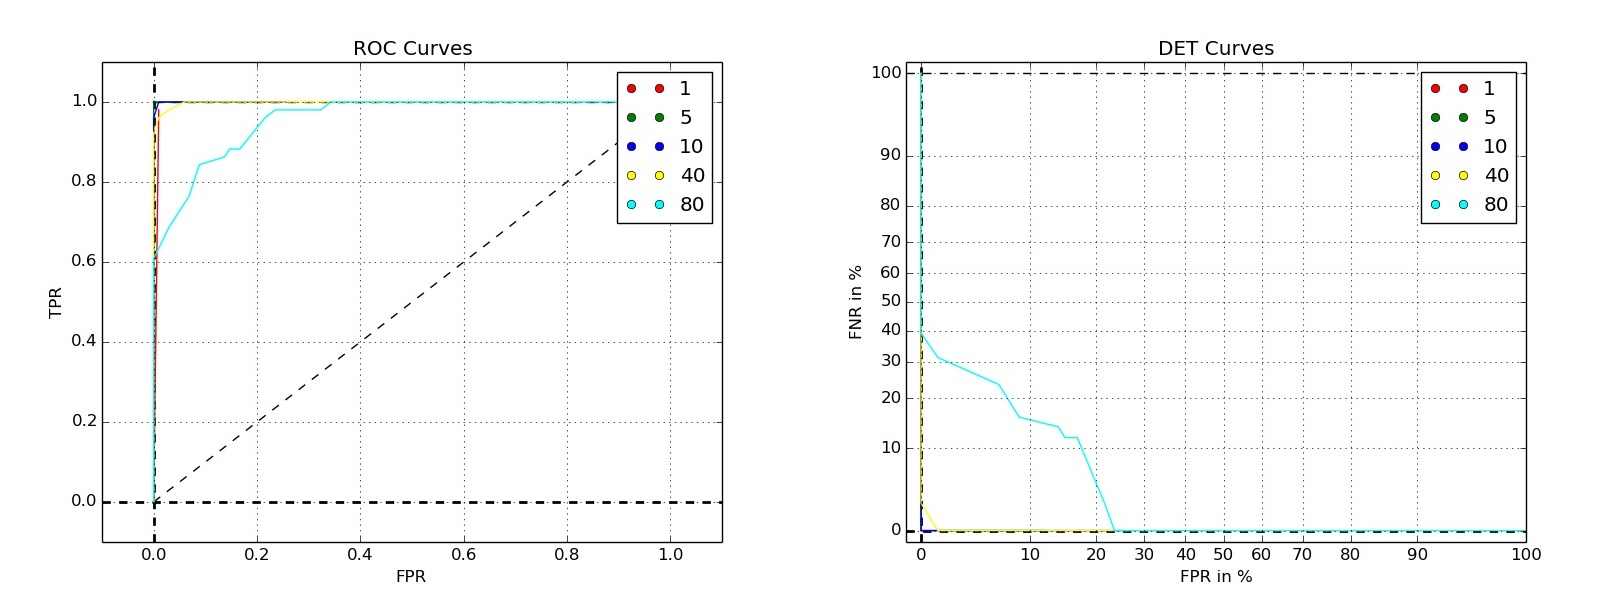
\includegraphics[width=\textwidth]{image_data/plots/roc_det.jpg}
\caption{$<\text{learning-rate}>\_<\text{epochs}>$}
\end{figure}


\begin{table}[h!]
\centering
\begin{tabular}{ |p{1.5cm}|p{1.5cm}|p{1.5cm}|p{1.5cm}|  }
\hline
\multicolumn{4}{|c|}{Confusion Matrix on Test Data} \\
\hline
 & Forest & Street & Highway \\
\hline
Forest & 46 & 2 & 1\\
Street & 0 & 42 & 1\\
Highway & 2 & 10 & 27\\
\hline
\end{tabular}
\end{table}

\end{document}